% !TEX root = main.tex

\section{Experimental Evaluation}\label{sec:experiments}


\begin{table*}[t]
	\large
	\centering
	\caption{Runtimes for four case studies.
		\textmd{Run times (in seconds) for computing open-loop controllers over the corresponding product spaces using ALTRO ($T_{g}^{\mathit{plan}}$), 
	number of input-state pairs of the finite abstraction for the largest ABCD task ($N_l$), 
	abstraction and synthesis times in SCOTS for that task (respectively $T_{l}^{\mathit{abs}}$ and $T_{l}^{\mathit{syn}}$), 
	number of input-state pairs of the finite state abstraction for the global ABCD ($N_g$), 
	abstraction and synthesis times for computing a global controller for the product system using SCOTS (respectively $T_{g}^{\mathit{abs}}$ and $T_{g}^{\mathit{syn}}$). \MZ{numbers are going to change again}
	% For local ABCD, the reported numbers correspond to the maximum value among all of the agents.
	}
		\label{tab:runtimes}
	}

	\renewcommand{\arraystretch}{1.2}
	%\setlength{\tabcolsep}{0.7em} % for the horizontal padding
	%\resizebox{1\columnwidth}{!}{
		\begin{tabular}{| l | S |S[table-format=+1.2e+1] S S|S[table-format=+1.2e+3] c c|}
			\hline
			Case-study	&	{Global planning}	&
			\multicolumn{3}{c|}{Local ABCD}	&	\multicolumn{3}{c|}{Global ABCD}\\
			
			&$T_{g}^{\mathit{plan}}$	&	$N_l$	&	$T_{l}^{\mathit{abs}}$	&	$T_{l}^{\mathit{syn}}$	&	$N_g$	&	$T_g^{\mathit{abs}}$	&	$T_g^{\mathit{syn}}$\\
			\hline
			
			Multi-drone path planning & 125 & 1.15e8 & 47.66  & 7.9	& 2.73e104	&	OOM	&	OOM \\
			
			\hline
			
			Crane and vehicle & 	0.65 & 8.56e8	&	511  & 91	&	2.16e18	&	OOM	&	OOM\\
			
			\hline
			
			Lane merging & 100 & 1.01e8	&	37.60  & 9.51	&	3.84e65	&	OOM	&	OOM\\
			\hline
			Multi-drone formation control & 163 & 4.02e8	&	69.78  & 13.6	&	3.7e59	&	OOM	&	OOM\\
			\hline
	\end{tabular}%}
\end{table*}

We have implemented our approach (as presented in Sec.~\ref{sec:problem}) in the tool called \tool, which is freely available online: https://github.com/MehrdadZareian/GMARA.
We evaluate the effectiveness of \tool on two distinct categories of problems: 
local reach-avoid problems with collision avoidance and global formation control problems. 
We consider four case studies: multi-drone path planning, crane and vehicle, lane merging, and multi-drone formation control. 
The design of nominal controller using ALTRO was performed on a laptop with core i7-4510u CPU at 3.10GHz, with 8GB of RAM.
The formal controller synthesis using SCOTS was performed on a cluster with 4 Intel Xeon E7-8857 v2 CPUs (48 cores in total) at 3GHz, with 1.5TB of RAM. 

In all of our case studies, the robots are moving in a two-dimensional shared workspace (related but not exactly the same as the robots' state spaces) that possibly has obstacles. 
Table~\ref{tab:runtimes} shows run times for different stages of each experiment. 
For local ABCD, the reported numbers correspond to the maximum value among all of the agents. 
This choice is due to the fact that feedback controllers for different agents can be computed independently 
in parallel over different machines. 
To provide a more fine-grained comparison,
Fig.~\ref{fig:box_plot} shows the variations of run times of the different local ABCD tasks for every experiment. 
We have excluded the crane and vehicle case study in the figure due to an expected large variance originating from different dynamics. 
%The corresponding numbers will be reported in the next section.
Notice that a higher number of input-state pairs does not necessarily result in a higher run time for local ABCD as the 
number of transitions and features of the parallel implementation can play a role. 
%
We compare \tool with the ABCD applied to the product system to satisfy the global specification. 
As reflected in Table~\ref{tab:runtimes}, memory requirement for the global ABCD exceeds our system's limit (1.5TB of RAM) in all of the experiments.
%
 %\MS{For reporting number of input-state pairs and run times of local ABCD we could report total, average or maximum values; currently, Tab.~\ref{tab:runtimes} contains maximum values (taken over all of the agents, corresponding to multi-machine implementation), while total and average values are reported in the body of the paper. Data will be unified once the decision is made.}
%Note that while reported numbers for local controller synthesis correspond to the total run times over all of the robots, significant reduction would be expected if abstraction and synthesis phases were parallelized.
%\begin{huge}

\begin{figure}[t]
	\centering
	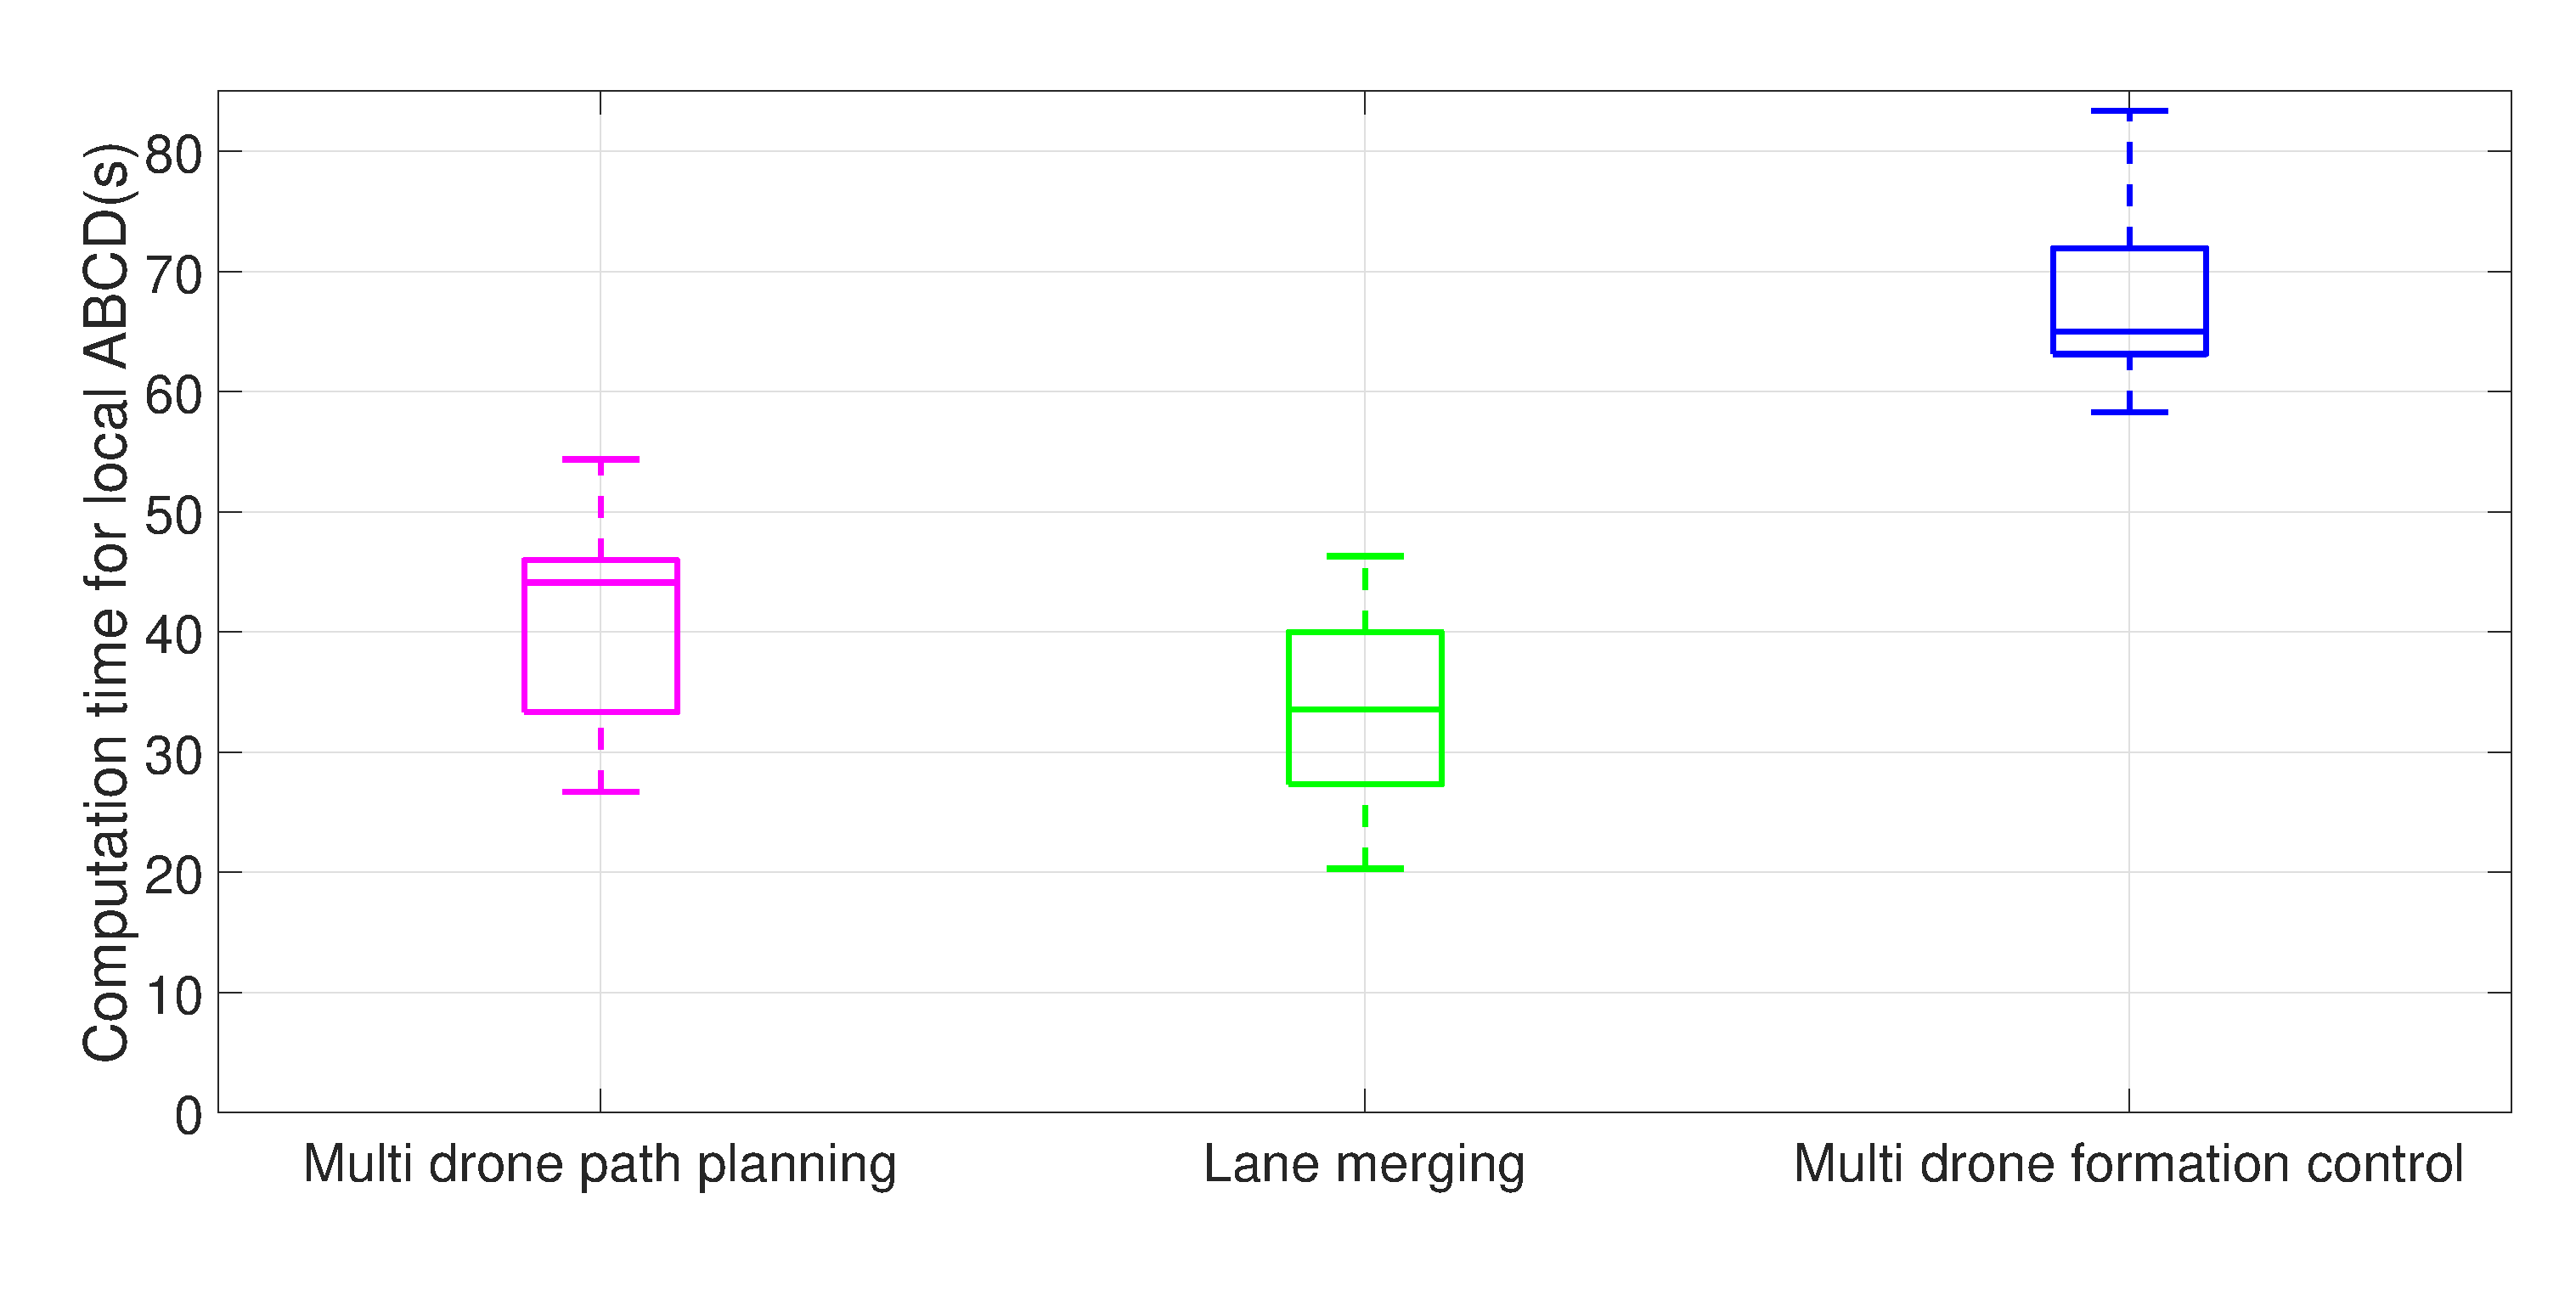
\includegraphics[width=0.45\textwidth]{figures/updated_box_plot.eps}
	\caption{Variations of run times of local ABCD among different agents for three case studies.}
	\label{fig:box_plot}
\end{figure}
%\vspace{-cm}
\begin{figure*}[t]
    \large
     \centering
     \begin{subfigure}[b]{0.2\textwidth}
         \centering
         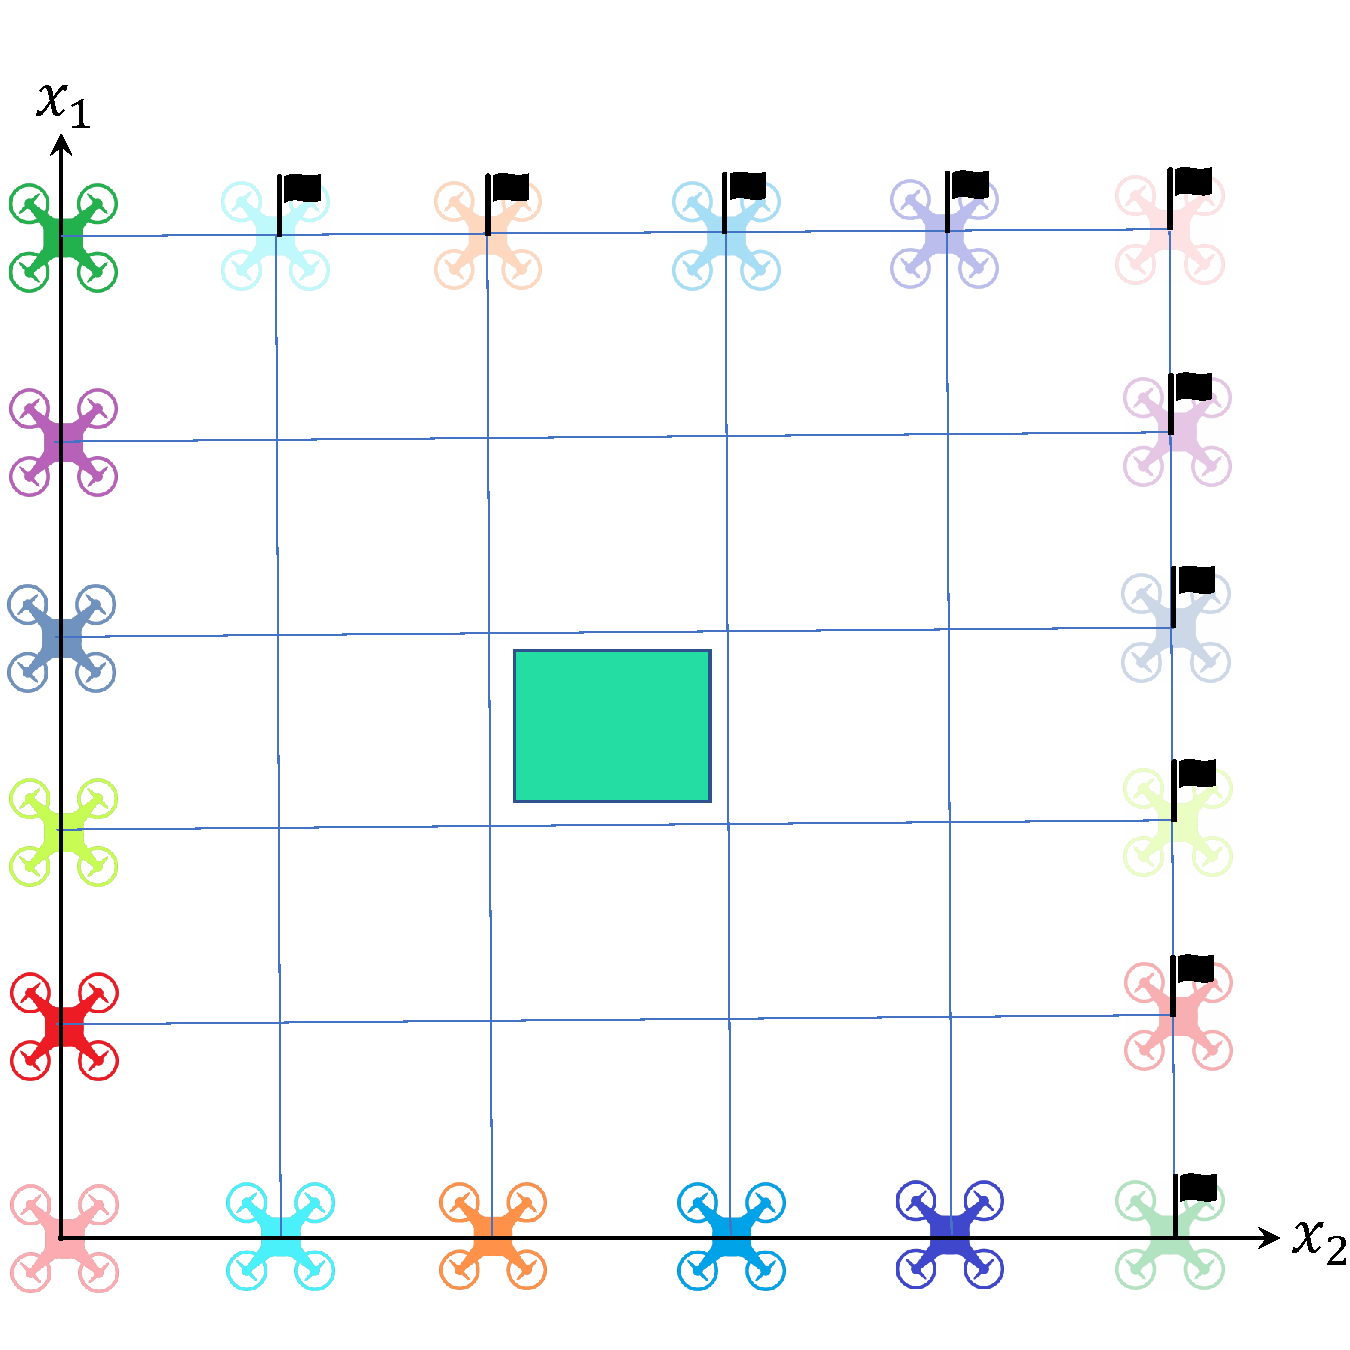
\includegraphics[width=\textwidth]{figures/multidrone.pdf}
         \caption{}
         \label{fig:MA}
     \end{subfigure}
     \hfill
     \begin{subfigure}[b]{0.39\textwidth}
         \centering
         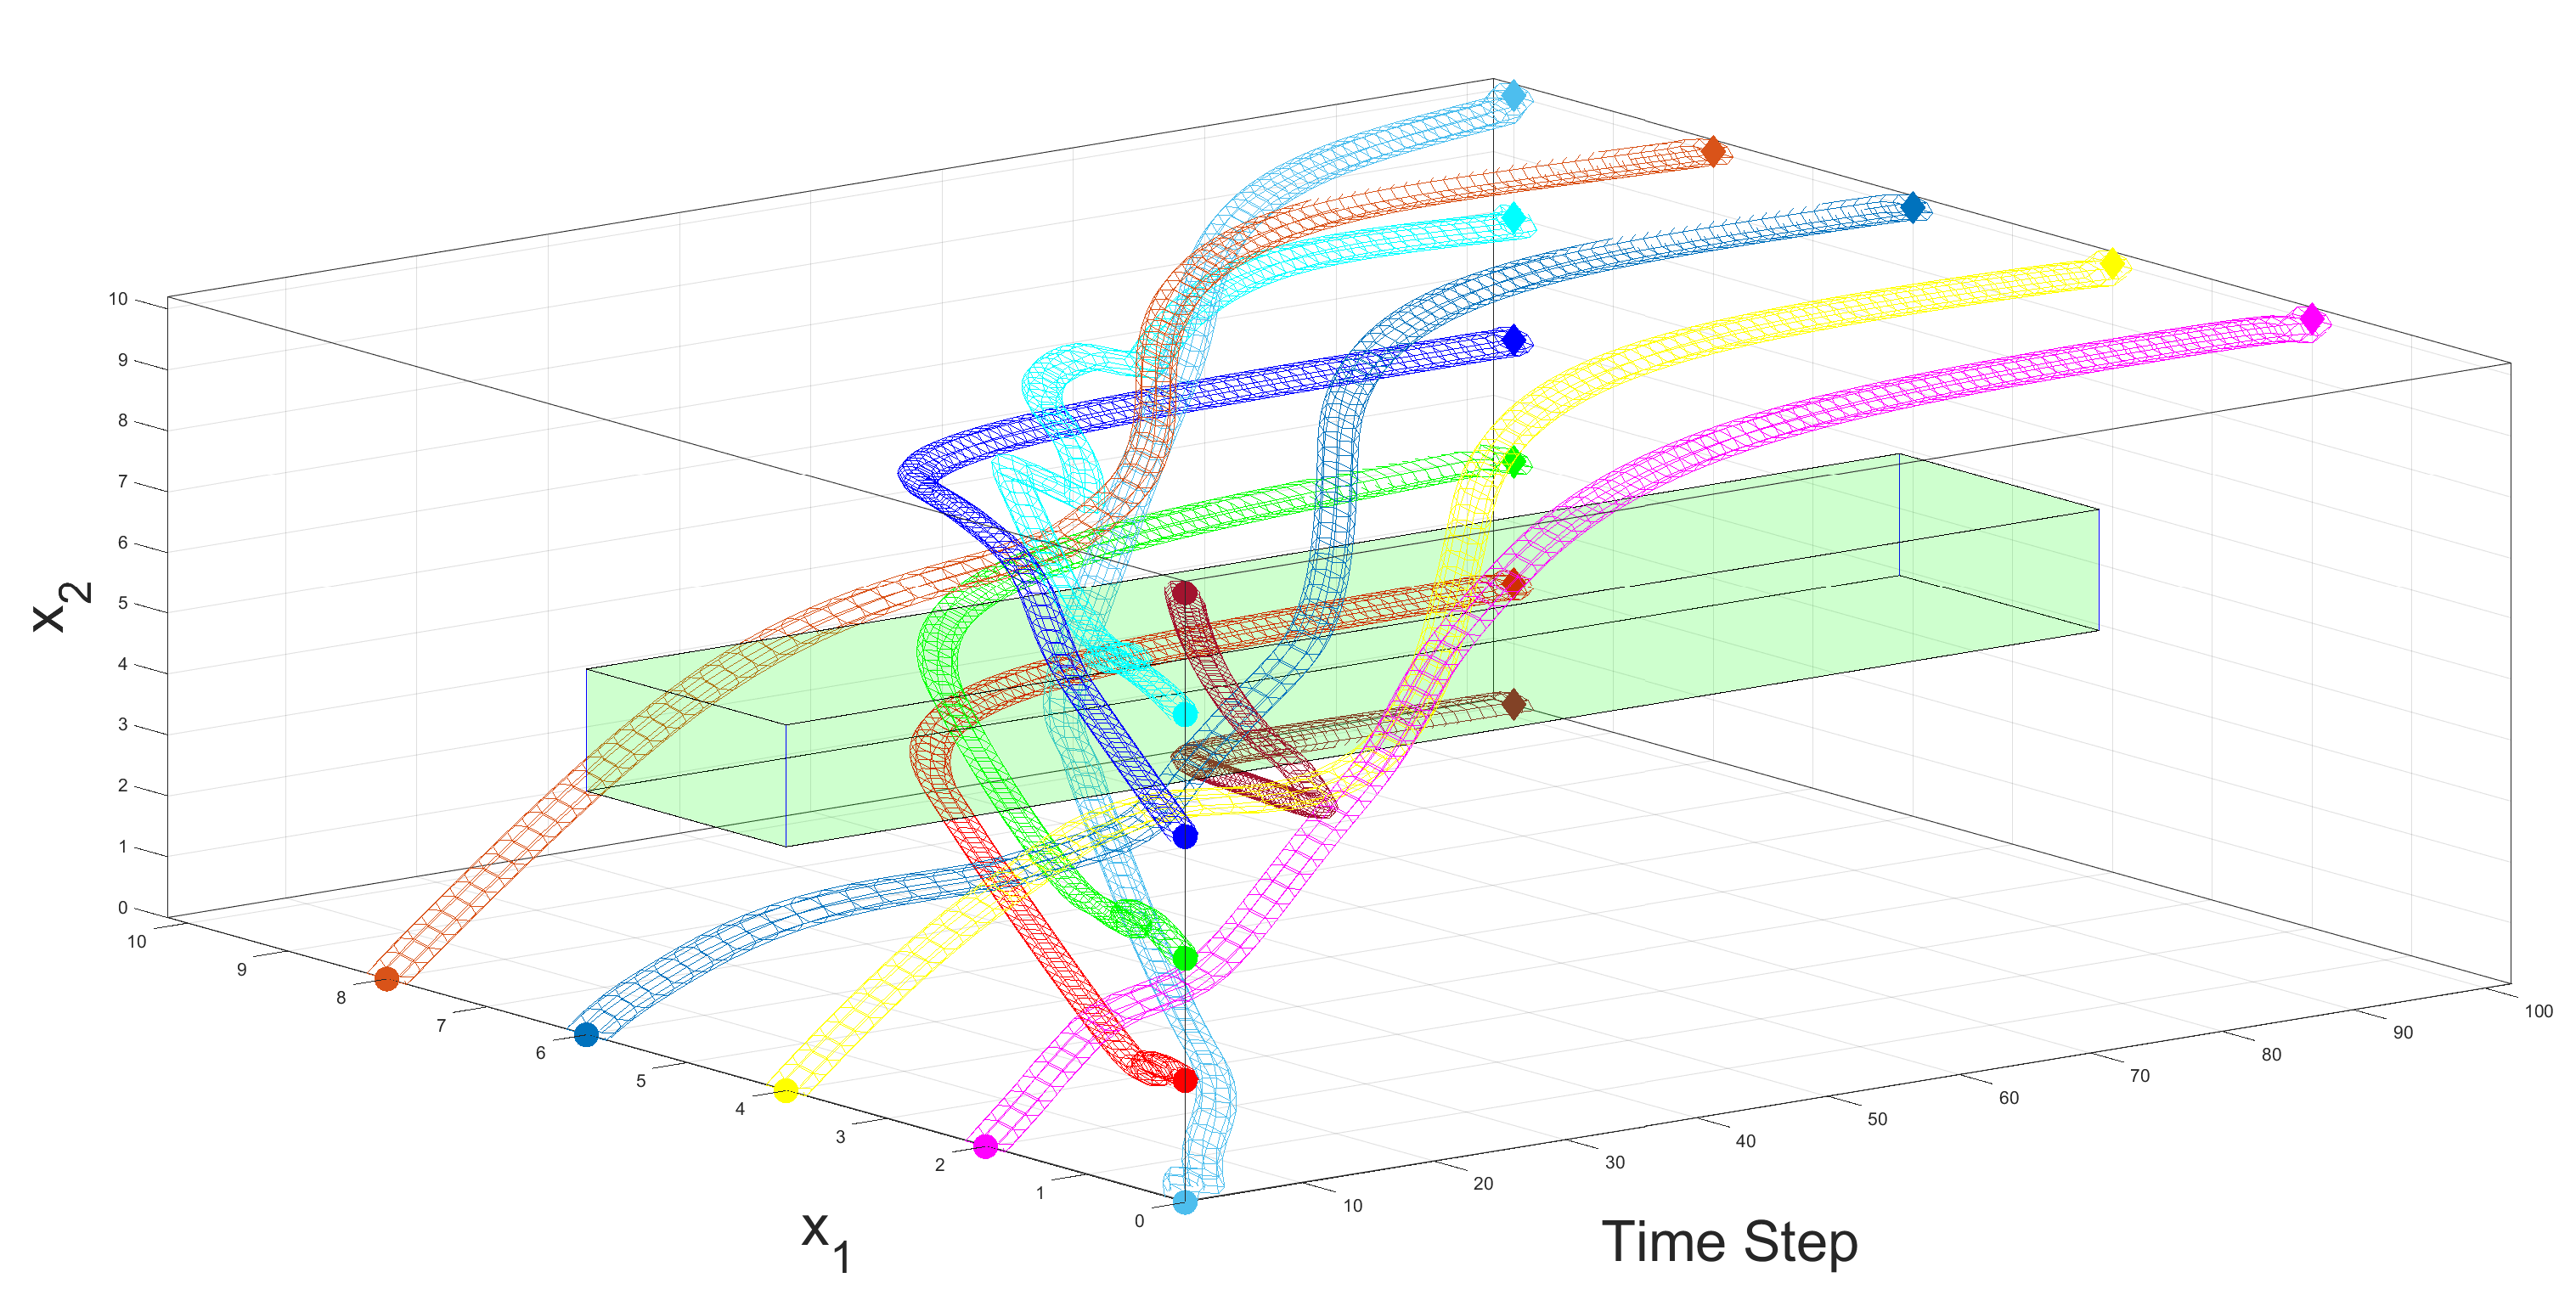
\includegraphics[width=\textwidth]{figures/tr10_final.eps}
         \caption{}
         \label{fig:3dtubes}
     \end{subfigure}
     \hfill
     \begin{subfigure}[b]{0.4\textwidth}
         \centering
         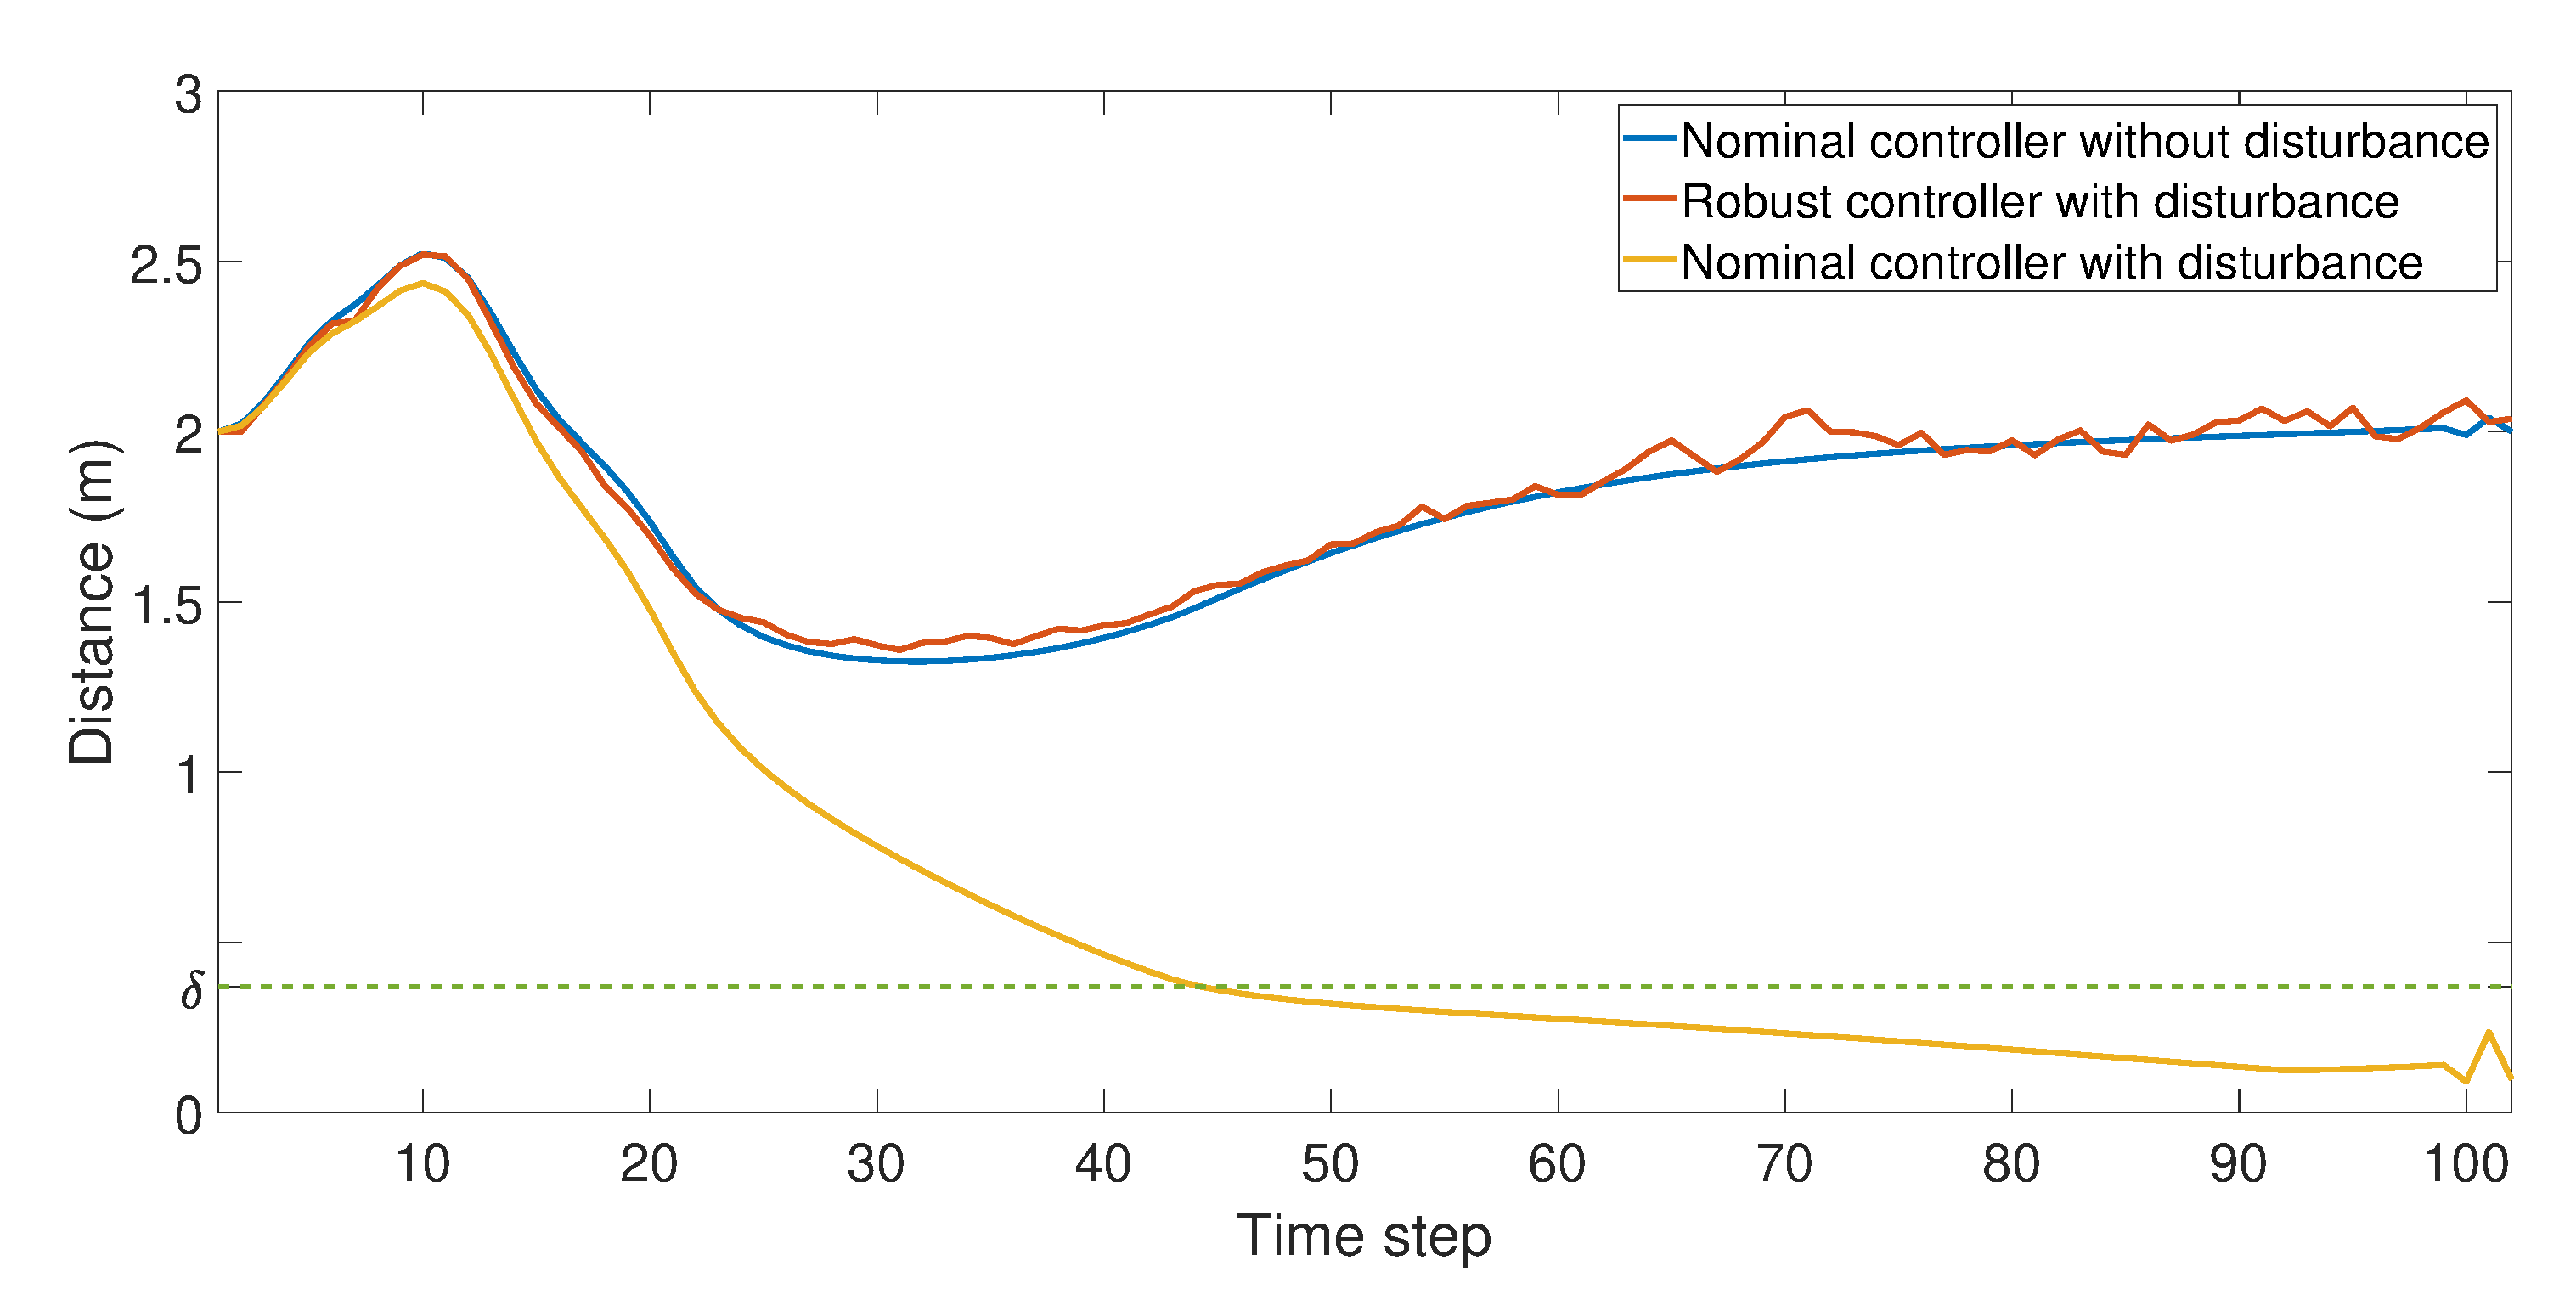
\includegraphics[width=\textwidth]{figures/multi_drone2.eps}
         \caption{}
         \label{fig:multi_drone_distance}
     \end{subfigure}
        \caption{(a) The mission map for the multi-drone path planning example, (b) Time-state space illustration of tubes enclosing nominal trajectories for the multi-drone path planning, and (c) Performance of open-loop and feedback controllers in regulating distance between two selected drones for disturbance-free and perturbed situations for the multi-drone path planning example.}
        \label{fig:three figures}
\end{figure*}

%\end{huge}
\subsection{Local reach-avoid with collision avoidance}
\label{sec:local reach-avoid}

We first consider situations when each robot has an individual reachability specification, 
and they need to ensure a minimum safe distance from each other and the obstacles.
% We show how this case can be captured using the problem description outlined in Sec.~\ref{sec:problem}.

Suppose $\set{\Sigma^i}$ 
% with $\Sigma^i=(X^i,x_\init^i,U^i,W^i,f^i)$ 
models a set of robots, 
$\goal^i\subseteq X^i$ are the individual goal sets, and $\delta \in \mathbb{R}_{>0}$ is a safety margin for collisions. 
\new{
We consider the robots as point objects.
In this case, the parameter $\delta$ can be seen as a constant greater than the radius of the bounding box around each robot, and by keeping a $\delta$ distance from the other robots and the obstacles, the robots can truly avoid collision in their physical domain.
The parameter $\delta$ can additionally take into account statutory minimum safe distances among the robots, such as in autonomous driving-like scenarios.
We emphasize that the choice of $\delta$ is completely independent of the choice of $\varepsilon$, where the latter is a robustness margin introduced to take into account the deviation of the system trajectories under external disturbances.
}
Suppose the specification requires that each robot $\Sigma^i$ eventually reaches $\goal^i$ 
while avoiding the obstacle $\obs\subseteq \reals^2$ and collision with robots by the margin $\delta$.
The global specification on the product system $\Sigma^\times$ 
is as follows:
\begin{itemize}
	\item The goal set $\goal\subseteq X^\times$ is defined as $\goal \coloneqq \goal^1\times \ldots \times \goal^N \subseteq X^\times$, and
	\item The avoid set $\avoid\subseteq X^\times$ is defined as 
		\begin{align}
% 			&\avoid \coloneqq\nonumber\\ 
				&\Set{ x^\times\in X^\times | 
					\begin{array}{c}
						\exists i\in [1;N]\;.\; d_\obs(x^i,\obs) \leq \delta\\
						\vee\\
						 \exists i,j\in [1;N]\;.\;i\neq j\;.\;d_\col\left(x^i,x^j\right)\leq\delta
					\end{array}},
		\end{align}
	where $x^i$ denotes the component of $x^\times$ corresponding to $\Sigma^i$, $d_\col(\cdot,\cdot)$ denotes a distance metric for measuring the geometric distance between positions of two systems located in the two-dimensional space, $d_\obs(\cdot,\cdot)$ denotes a distance metric for measuring the geometric distance between position of one system and the obstacle $\obs\subseteq \reals^2$.
\end{itemize}
%
% Once the sets $\goal$ and $\avoid$ are obtained as above, we can use Alg.~\ref{alg:main} to find the set of feedback controllers $\set{C^i}$.
%

\new{
In this category of problems, we apply \tool to three multi-robot case studies, namely a multi-drone path planning problem (Fig.~\ref{fig:three figures}), a crane and a vehicle problem (Fig.~\ref{fig:cr_and_lft}), and a lane merging problem (Fig.~\ref{fig:merge}-\ref{fig:merging_distance}); the detailed models for the systems and their different parameters have been presented in Sec.~\ref{sec:Multirobot}-\ref{sec:lane merging} in the appendix, and the performance of \tool for these experiments have been summarized in the first three rows on Table~\ref{tab:runtimes}.
}
%\textcolor{red}{



\begin{figure}
	\centering
	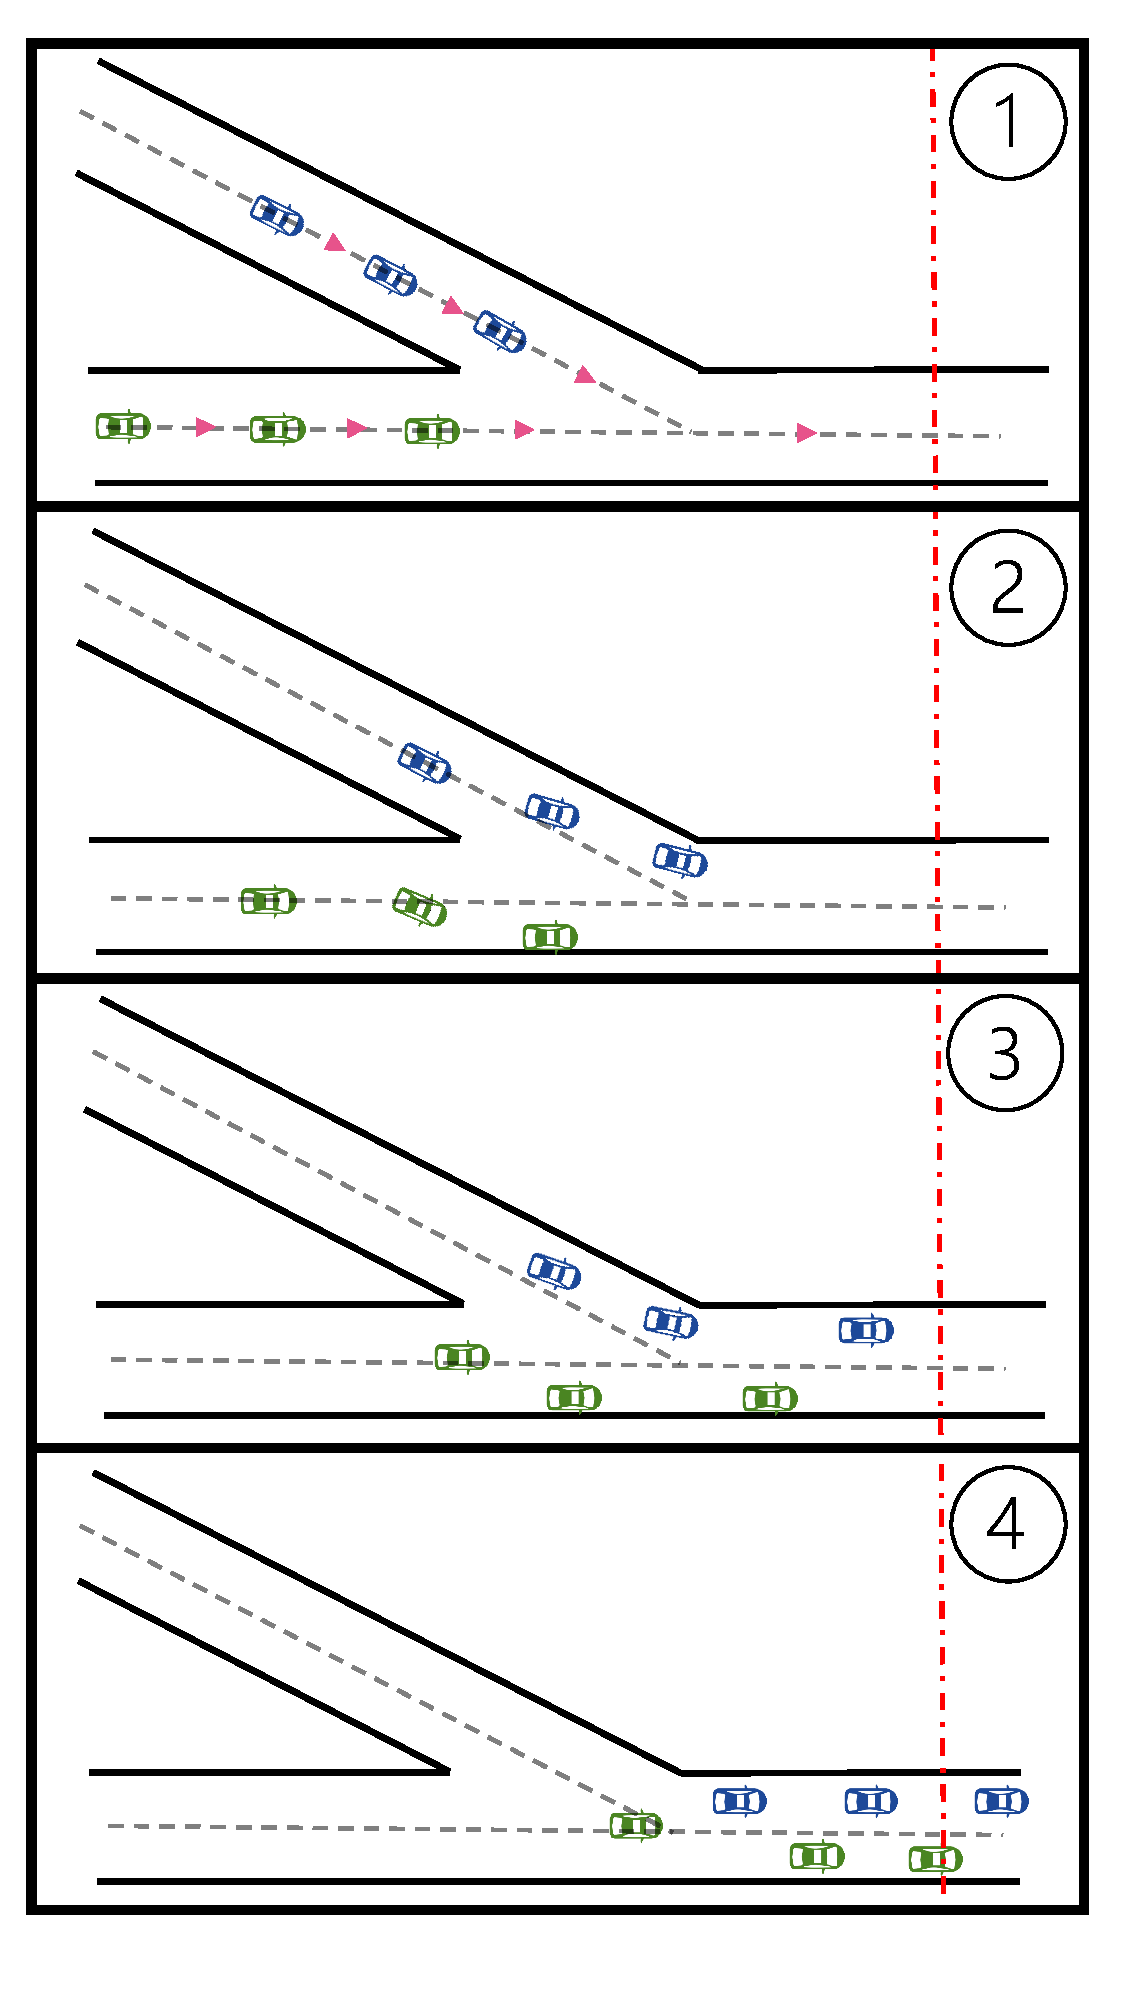
\includegraphics[scale=.21]{figures/merge_updated.pdf}
	\caption{Illustration of a sample trajectory generated by formally guaranteed controllers for the lane merging example}
	\label{fig:merge}
\vspace*{-0.2cm}
\end{figure}

%\vspace{-1cm}

\begin{figure}
	\centering
	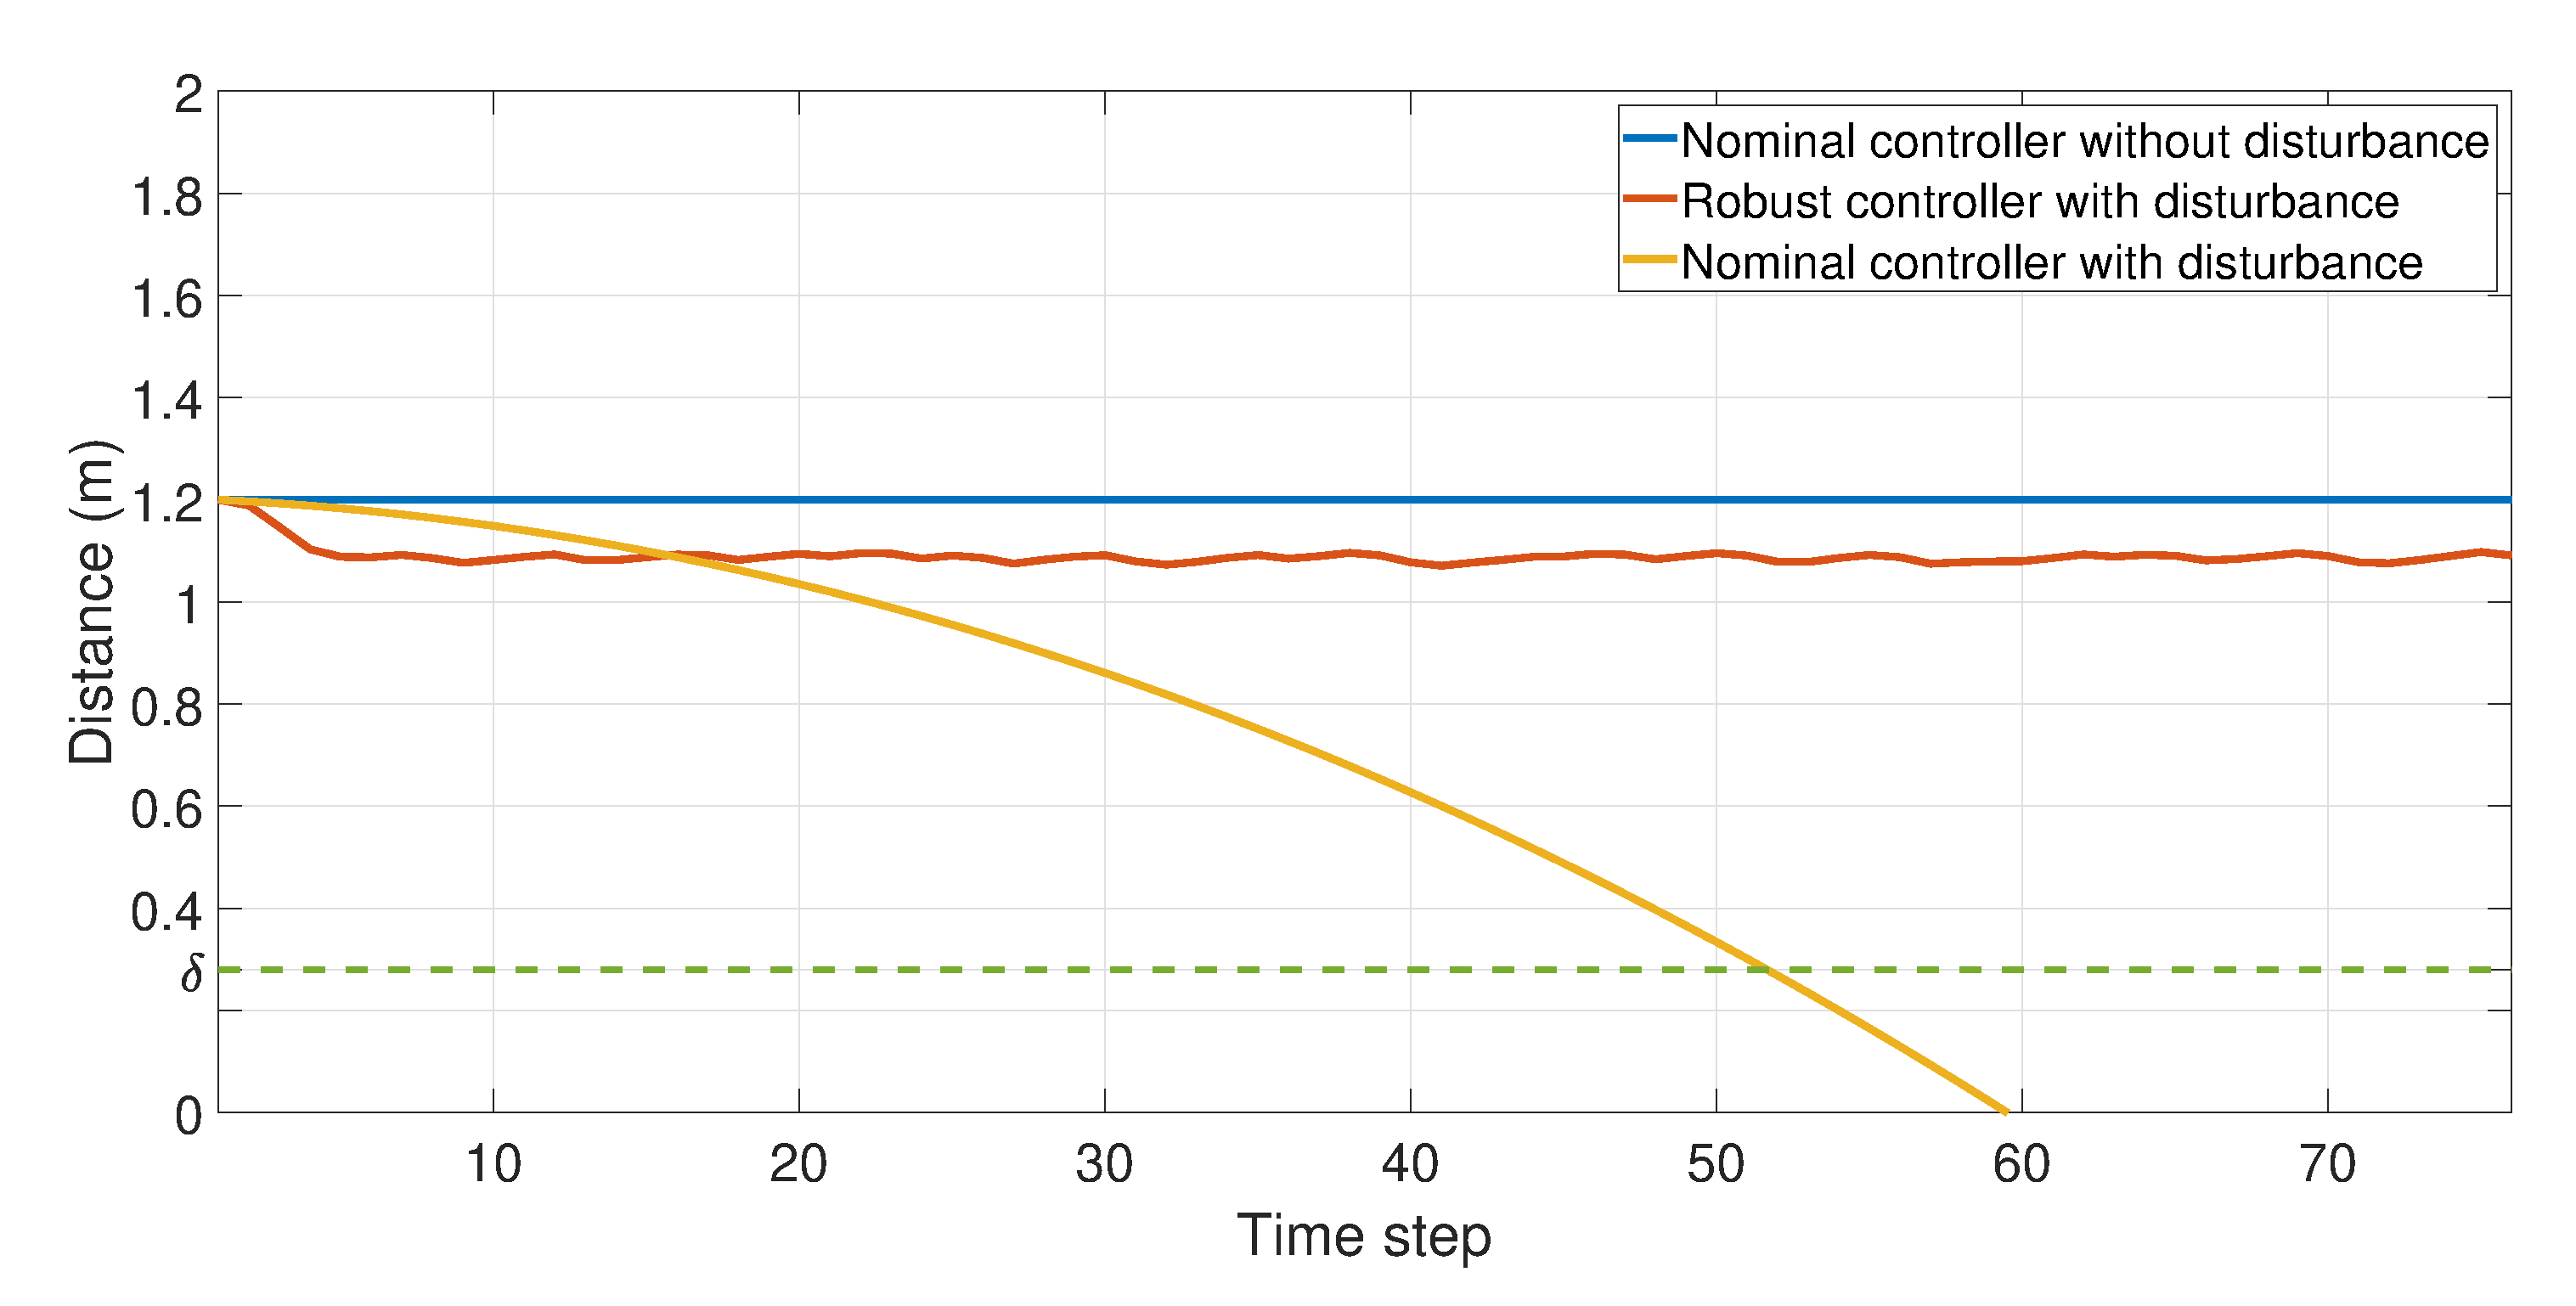
\includegraphics[width=0.45\textwidth]{figures/Merge_plot2.eps}
	\caption{Comparison of open-loop and feedback controllers for the lane merging example}
	\label{fig:merging_distance}
\vspace*{-0.3cm}
\end{figure}

\subsection{Global formation control problem}\label{sec:global formation control}

The second category of examples are about maintaining a global formation while satisfying a set of reach-avoid specifications.
We show how the formation control problem can be expressed using a static obstacle $\avoid$ on the product state space $X^\times$.

Let us first formalize the notion of \emph{formation}.
Let $\Set{\Sigma^i=(X^i,x_\init^i,U^i,W^i,f^i)}$ be a set of robots.
A \emph{formation constraint} is a set $\Set{\lambda^{i,j}\in \mathbb{R}}_{i,j\in [1;N]}$ where every $\lambda^{i,j}$ specifies the relative \emph{Euclidean} 
distance between the projections of state of robot $\Sigma^i$ and robot $\Sigma^j$.%\RM{undef:} over the shared output space $Y$.
%(We use euclidean distance to define formation, as opposed to the distance $D$ used in the rest of the paper, to allow rotation of the formation while moving.)

Now suppose $\goal^i\subseteq X^i$ are the individual goal states, $\obs\subset \reals^2$ is a common obstacle % in the \RM{undef:} output space, 
$\delta \in \mathbb{R}_{>0}$ is a safety margin, and $\mu\in \mathbb{R}_{>0}$ is a tolerance margin for the formation constraint.
The formation control problem then asks to generate controllers $\set{C_i}$ such that every robot $\Sigma^i$ eventually reaches $\goal^i$ while avoiding $\obs$ 
by the margin $\delta$, as well as while making sure that the \emph{Euclidean} distance between robots $\Sigma^i$ and $\Sigma^j$ is in the range $\lambda^{i,j} \pm \mu$.
Essentially the tolerance margin $\mu$ is to account for the possible slight deviations due to disturbances experienced by the robots. 
Notice that since the robots have their own goals but at the same time they need to ``stay close'' to their neighboring robots in the formation for the entire period, 
they might first need to accompany the other robots to their goals, before being accompanied by them to reach their own goal.
%
We can express the formation control problem in the product state space as follows:
\begin{itemize}
	\item The goal set $\goal\!\subseteq\! X^\times$ is defined as $\goal\!\coloneqq\! \goal^1\!\times \ldots \times\! \goal^N$, and
	\item The avoid set $\avoid\subseteq X^\times$ is 
		\begin{align}
%			&\avoid \coloneqq\nonumber\\ 
			&\Set{ x^\times\in X^\times | 
				\begin{array}{c}
					\exists i\in [1;N]\;.\; D(x^i,\obs) \leq \delta\\
					\vee\\
					\exists i,j\in [1;N]\;.\; i\neq j\;.\; d\left(x^i,x^j\right)\notin\lambda^{i,j}\pm \mu
			\end{array}},					
		\end{align}
\end{itemize}
where the last disjunction in the definition of $\avoid$ is the restriction required for maintaining the formation, and the rest are 
same as in Sec.~\ref{sec:local reach-avoid}.
% Once the sets $\goal$ and $\avoid$ are obtained as above, we can use Alg.~\ref{alg:main} to find the set of feedback controllers $\set{C^i}$.

%\todo{The example goes here...}

\new{
We performed a multi-drone formation control experiment (Fig.~\ref{fig:formation_ex}-\ref{fig:formation_distance}), where the models of the systems and the parameters used have been reported in Sec.~\ref{subsec:formation_control} in the appendix.
The performance of \tool for this experiment has been reported in the last row of Table~\ref{tab:runtimes}.
}

 \begin{figure}[t]
	\centering
	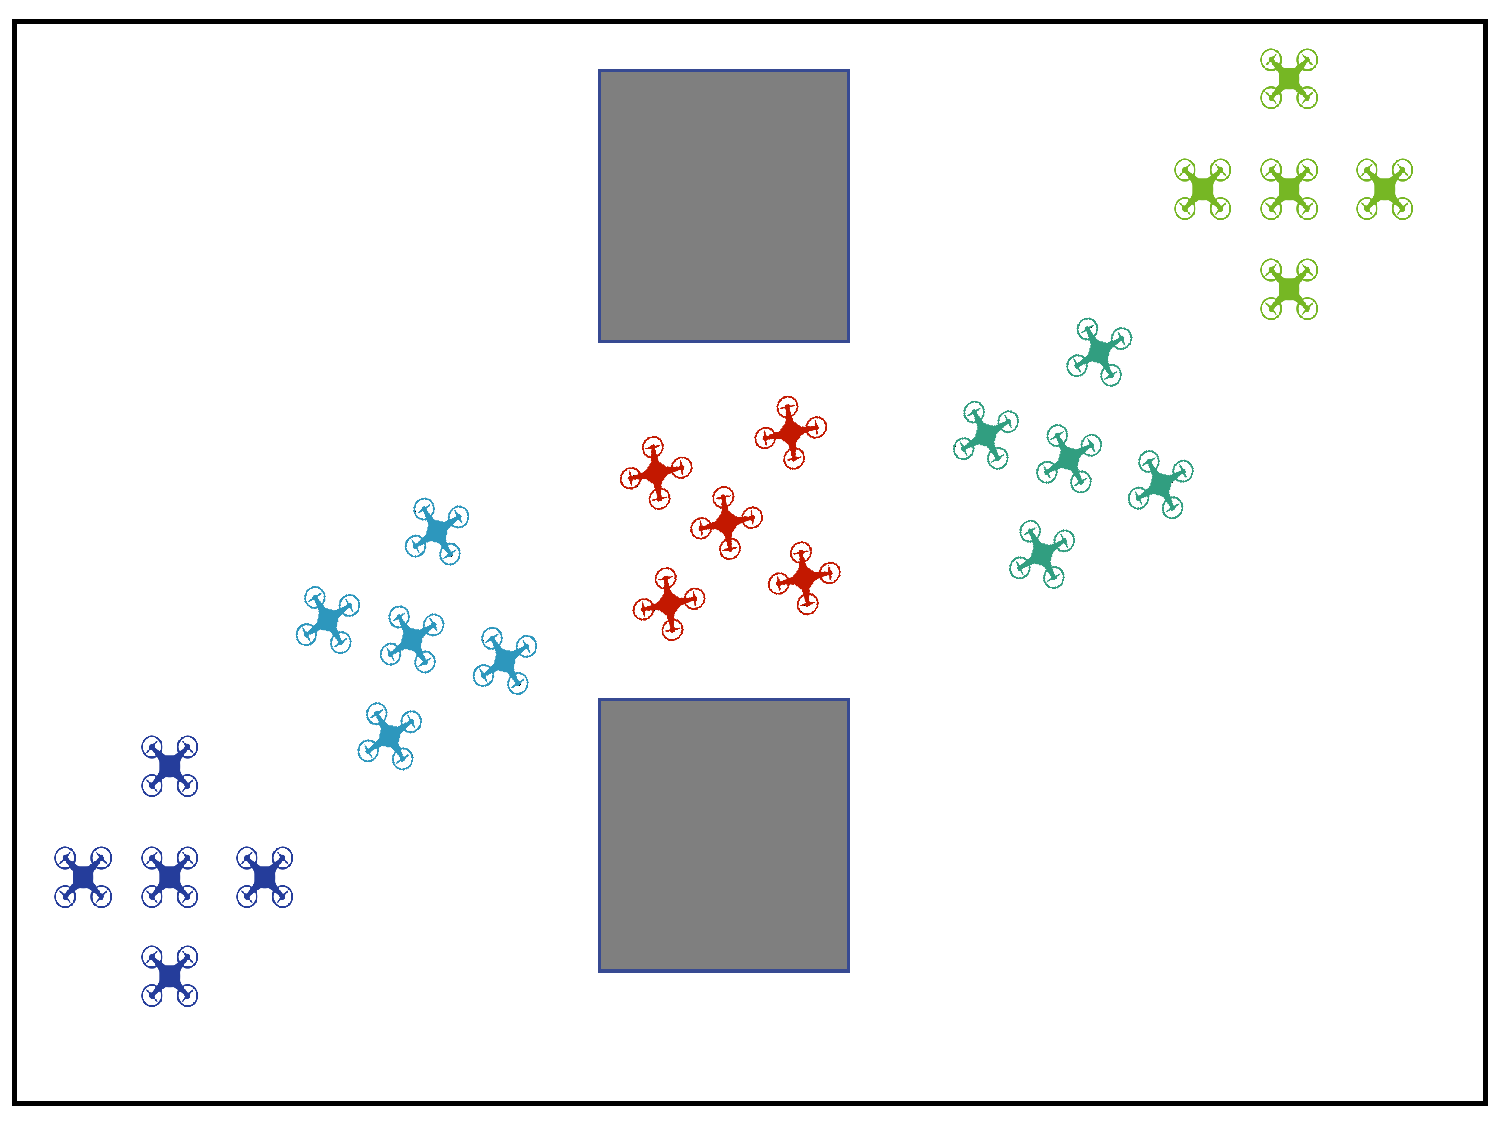
\includegraphics[scale=0.22]{figures/formation.pdf}
	\caption{Illustration of a sample trajectory generated by the feedback controllers for the formation control example}
	\label{fig:formation_ex}
\end{figure}

\begin{figure}[t]
	\centering
	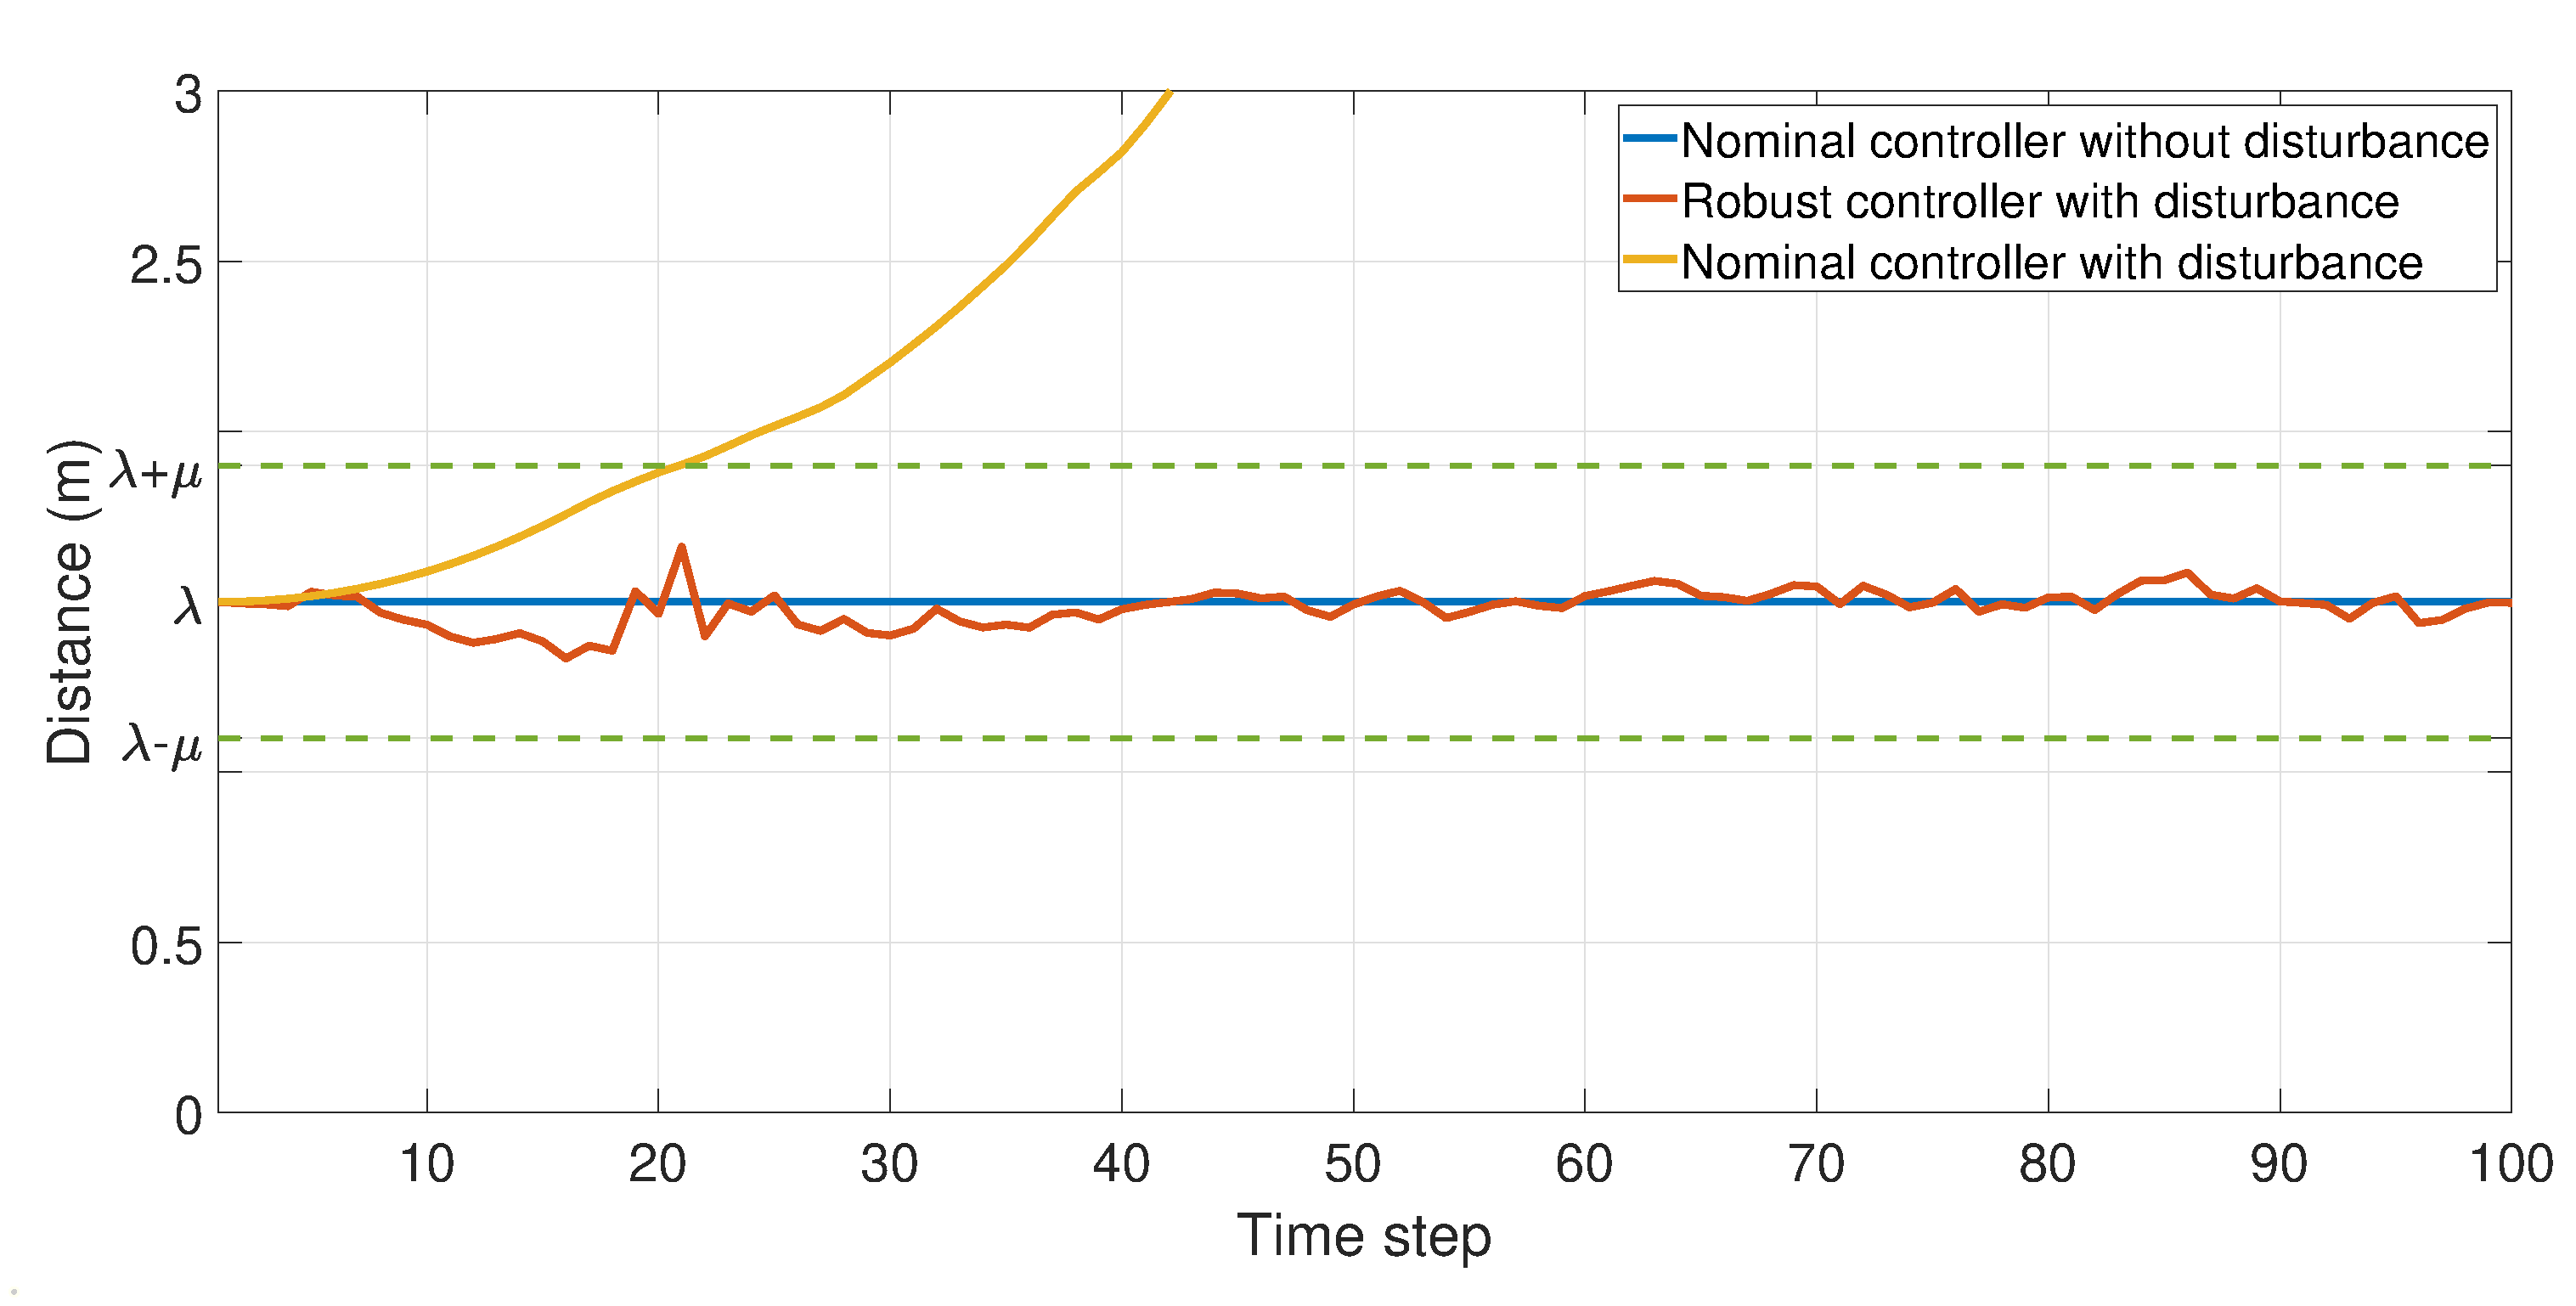
\includegraphics[width=0.45\textwidth]{figures/formation_dist2.eps}
	\caption{Comparison of open-loop and feedback controllers for the formation control example}
	\label{fig:formation_distance}
\vspace*{-0.5cm}
\end{figure}
 

%Note that $\delta_{col} > \varepsilon$.
%We use SCOTS in order to synthesize (local) feedback controllers that guarantee reachability, formation control and obstacle/collision avoidance in the presence of bounded disturbance such that $|W|\leq \begin{bmatrix}??&??&??\end{bmatrix}^T$. 
%We consider state and input spaces to be $X=[??:??]^2\times[??,??]$ and
%$U=[??,??]^2$, respectively. Choosing state and input partition sizes $\eta_{X}=[??,??,??]^T$ and
%$\eta_{U}=[??,??]^T$ results in $\hat X$ and $\hat U$ with $??\times ??$ and $??$ points. As we explained in Sec.~\ref{sec:tracking}, we compute the transition system over inter-tube space which has $|\hat P|=??\times ??$ points in this example.%The bound over additive disturbance is set to be $\begin{bmatrix}0.03&0.03&0.03&0\end{bmatrix}^T$. 
%Given the above settings, SCOTS computes abstraction in $??$ minutes for all the drones and synthesizes controllers in about $??$ minutes (in average, abstraction takes $??$ seconds and synthesis takes $??$ seconds). 
%\section{Present Challenges}
%
%\begin{enumerate}
%	\item In some examples, it was necessary to consider a larger control input space for the SCOTS part, than what was used in the ALTRO part.
%	Otherwise, the SCOTS would not be able to track the nominal trajectory within the given precision using any level of discretization. 
%	\item For the ship example, applying the largest disturbance with which SCOTS is able to compute a controller, the trajectory resulted from using the open loop controller does not leave  $\varepsilon-$tube around it; in general magnitude of disturbance for which SCOTS can find a controller is relatively small for most of examples that we have tried.
%\end{enumerate}









